\documentclass{report}

%%%%%%%%%%%%%%%%%%%%%%%%%%%%%%%%
% PACKAGE IMPORTS
%%%%%%%%%%%%%%%%%%%%%%%%%%%%%%%%%


\usepackage[tmargin=2cm,rmargin=1in,lmargin=1in,margin=0.85in,bmargin=2cm,footskip=.2in]{geometry}
\usepackage{amsmath,amsfonts,amsthm,amssymb,mathtools}
\usepackage[varbb]{newpxmath}
\usepackage{xfrac}
\usepackage[makeroom]{cancel}
\usepackage{mathtools}
\usepackage{bookmark}
\usepackage{enumitem}
\usepackage{hyperref,theoremref}
\hypersetup{
	pdftitle={Assignment},
	colorlinks=true, linkcolor=doc!90,
	bookmarksnumbered=true,
	bookmarksopen=true
}
\usepackage[most,many,breakable]{tcolorbox}
\usepackage{xcolor}
\usepackage{varwidth}
\usepackage{varwidth}
\usepackage{etoolbox}
%\usepackage{authblk}
\usepackage{nameref}
\usepackage{multicol,array}
\usepackage{tikz-cd}
\usepackage{tikz-3dplot}
\usepackage[ruled,vlined,linesnumbered]{algorithm2e}
\usepackage{comment} % enables the use of multi-line comments (\ifx \fi) 
\usepackage{import}
\usepackage{xifthen}
\usepackage{pdfpages}
\usepackage{transparent}
\usepackage{graphicx} % <-- Added package to handle graphics
\usepackage{xcolor}
\usepackage{pgfplots}
\usepackage{minted}
\definecolor{pastelFDF7C3}{HTML}{FDF7C3}
\pgfplotsset{compat=newest}
\usepgfplotslibrary{colormaps}


\newcommand\mycommfont[1]{\footnotesize\ttfamily\textcolor{blue}{#1}}
\SetCommentSty{mycommfont}
\newcommand{\incfig}[1]{%
    \def\svgwidth{\columnwidth}
    \import{./figures/}{#1.pdf_tex}
}

\usepackage{tikzsymbols}
\renewcommand\qedsymbol{$\Laughey$}


%\usepackage{import}
%\usepackage{xifthen}
%\usepackage{pdfpages}
%\usepackage{transparent}


%%%%%%%%%%%%%%%%%%%%%%%%%%%%%%
% SELF MADE COLORS
%%%%%%%%%%%%%%%%%%%%%%%%%%%%%%



\definecolor{myg}{RGB}{56, 140, 70}
\definecolor{myb}{RGB}{45, 111, 177}
\definecolor{myr}{RGB}{199, 68, 64}
\definecolor{mytheorembg}{HTML}{F2F2F9}
\definecolor{mytheoremfr}{HTML}{00007B}
\definecolor{mylenmabg}{HTML}{FFFAF8}
\definecolor{mylenmafr}{HTML}{983b0f}
\definecolor{mypropbg}{HTML}{f2fbfc}
\definecolor{mypropfr}{HTML}{191971}
\definecolor{myexamplebg}{HTML}{F2FBF8}
\definecolor{myexamplefr}{HTML}{88D6D1}
\definecolor{myexampleti}{HTML}{2A7F7F}
\definecolor{mydefinitbg}{HTML}{E5E5FF}
\definecolor{mydefinitfr}{HTML}{3F3FA3}
\definecolor{notesgreen}{RGB}{0,162,0}
\definecolor{myp}{RGB}{197, 92, 212}
\definecolor{mygr}{HTML}{2C3338}
\definecolor{myred}{RGB}{127,0,0}
\definecolor{myyellow}{RGB}{169,121,69}
\definecolor{myexercisebg}{HTML}{F2FBF8}
\definecolor{myexercisefg}{HTML}{88D6D1}


%%%%%%%%%%%%%%%%%%%%%%%%%%%%
% TCOLORBOX SETUPS
%%%%%%%%%%%%%%%%%%%%%%%%%%%%

\setlength{\parindent}{1cm}
%================================
% THEOREM BOX
%================================

\tcbuselibrary{theorems,skins,hooks}
\newtcbtheorem[number within=section]{Theorem}{Theorem}
{%
	enhanced,
	breakable,
	colback = mytheorembg,
	frame hidden,
	boxrule = 0sp,
	borderline west = {2pt}{0pt}{mytheoremfr},
	sharp corners,
	detach title,
	before upper = \tcbtitle\par\smallskip,
	coltitle = mytheoremfr,
	fonttitle = \bfseries\sffamily,
	description font = \mdseries,
	separator sign none,
	segmentation style={solid, mytheoremfr},
}
{th}

\tcbuselibrary{theorems,skins,hooks}
\newtcbtheorem[number within=chapter]{theorem}{Theorem}
{%
	enhanced,
	breakable,
	colback = mytheorembg,
	frame hidden,
	boxrule = 0sp,
	borderline west = {2pt}{0pt}{mytheoremfr},
	sharp corners,
	detach title,
	before upper = \tcbtitle\par\smallskip,
	coltitle = mytheoremfr,
	fonttitle = \bfseries\sffamily,
	description font = \mdseries,
	separator sign none,
	segmentation style={solid, mytheoremfr},
}
{th}


\tcbuselibrary{theorems,skins,hooks}
\newtcolorbox{Theoremcon}
{%
	enhanced
	,breakable
	,colback = mytheorembg
	,frame hidden
	,boxrule = 0sp
	,borderline west = {2pt}{0pt}{mytheoremfr}
	,sharp corners
	,description font = \mdseries
	,separator sign none
}

%================================
% Corollery
%================================
\tcbuselibrary{theorems,skins,hooks}
\newtcbtheorem[number within=section]{Corollary}{Corollary}
{%
	enhanced
	,breakable
	,colback = myp!10
	,frame hidden
	,boxrule = 0sp
	,borderline west = {2pt}{0pt}{myp!85!black}
	,sharp corners
	,detach title
	,before upper = \tcbtitle\par\smallskip
	,coltitle = myp!85!black
	,fonttitle = \bfseries\sffamily
	,description font = \mdseries
	,separator sign none
	,segmentation style={solid, myp!85!black}
}
{th}
\tcbuselibrary{theorems,skins,hooks}
\newtcbtheorem[number within=chapter]{corollary}{Corollary}
{%
	enhanced
	,breakable
	,colback = myp!10
	,frame hidden
	,boxrule = 0sp
	,borderline west = {2pt}{0pt}{myp!85!black}
	,sharp corners
	,detach title
	,before upper = \tcbtitle\par\smallskip
	,coltitle = myp!85!black
	,fonttitle = \bfseries\sffamily
	,description font = \mdseries
	,separator sign none
	,segmentation style={solid, myp!85!black}
}
{th}


%================================
% LENMA
%================================

\tcbuselibrary{theorems,skins,hooks}
\newtcbtheorem[number within=section]{Lenma}{Lenma}
{%
	enhanced,
	breakable,
	colback = mylenmabg,
	frame hidden,
	boxrule = 0sp,
	borderline west = {2pt}{0pt}{mylenmafr},
	sharp corners,
	detach title,
	before upper = \tcbtitle\par\smallskip,
	coltitle = mylenmafr,
	fonttitle = \bfseries\sffamily,
	description font = \mdseries,
	separator sign none,
	segmentation style={solid, mylenmafr},
}
{th}

\tcbuselibrary{theorems,skins,hooks}
\newtcbtheorem[number within=chapter]{lenma}{Lenma}
{%
	enhanced,
	breakable,
	colback = mylenmabg,
	frame hidden,
	boxrule = 0sp,
	borderline west = {2pt}{0pt}{mylenmafr},
	sharp corners,
	detach title,
	before upper = \tcbtitle\par\smallskip,
	coltitle = mylenmafr,
	fonttitle = \bfseries\sffamily,
	description font = \mdseries,
	separator sign none,
	segmentation style={solid, mylenmafr},
}
{th}


%================================
% PROPOSITION
%================================

\tcbuselibrary{theorems,skins,hooks}
\newtcbtheorem[number within=section]{Prop}{Proposition}
{%
	enhanced,
	breakable,
	colback = mypropbg,
	frame hidden,
	boxrule = 0sp,
	borderline west = {2pt}{0pt}{mypropfr},
	sharp corners,
	detach title,
	before upper = \tcbtitle\par\smallskip,
	coltitle = mypropfr,
	fonttitle = \bfseries\sffamily,
	description font = \mdseries,
	separator sign none,
	segmentation style={solid, mypropfr},
}
{th}

\tcbuselibrary{theorems,skins,hooks}
\newtcbtheorem[number within=chapter]{prop}{Proposition}
{%
	enhanced,
	breakable,
	colback = mypropbg,
	frame hidden,
	boxrule = 0sp,
	borderline west = {2pt}{0pt}{mypropfr},
	sharp corners,
	detach title,
	before upper = \tcbtitle\par\smallskip,
	coltitle = mypropfr,
	fonttitle = \bfseries\sffamily,
	description font = \mdseries,
	separator sign none,
	segmentation style={solid, mypropfr},
}
{th}


%================================
% CLAIM
%================================

\tcbuselibrary{theorems,skins,hooks}
\newtcbtheorem[number within=section]{claim}{Claim}
{%
	enhanced
	,breakable
	,colback = myg!10
	,frame hidden
	,boxrule = 0sp
	,borderline west = {2pt}{0pt}{myg}
	,sharp corners
	,detach title
	,before upper = \tcbtitle\par\smallskip
	,coltitle = myg!85!black
	,fonttitle = \bfseries\sffamily
	,description font = \mdseries
	,separator sign none
	,segmentation style={solid, myg!85!black}
}
{th}



%================================
% Exercise
%================================

\tcbuselibrary{theorems,skins,hooks}
\newtcbtheorem[number within=section]{Exercise}{Exercise}
{%
	enhanced,
	breakable,
	colback = myexercisebg,
	frame hidden,
	boxrule = 0sp,
	borderline west = {2pt}{0pt}{myexercisefg},
	sharp corners,
	detach title,
	before upper = \tcbtitle\par\smallskip,
	coltitle = myexercisefg,
	fonttitle = \bfseries\sffamily,
	description font = \mdseries,
	separator sign none,
	segmentation style={solid, myexercisefg},
}
{th}

\tcbuselibrary{theorems,skins,hooks}
\newtcbtheorem[number within=chapter]{exercise}{Exercise}
{%
	enhanced,
	breakable,
	colback = myexercisebg,
	frame hidden,
	boxrule = 0sp,
	borderline west = {2pt}{0pt}{myexercisefg},
	sharp corners,
	detach title,
	before upper = \tcbtitle\par\smallskip,
	coltitle = myexercisefg,
	fonttitle = \bfseries\sffamily,
	description font = \mdseries,
	separator sign none,
	segmentation style={solid, myexercisefg},
}
{th}

%================================
% EXAMPLE BOX (Lighter Pastel Purple)
%================================

\definecolor{pastelExampleBg}{HTML}{70AF85} % Base pastel color
\definecolor{greenPast}{HTML}{86C8BC} % Base pastel color
\colorlet{myexamplebg}{pastelExampleBg!25!white} % Mix with white for a pastel color
\colorlet{myexamplefr}{pastelExampleBg!85!white} % Use the same mix for the frame
\colorlet{myexampleti}{greenPast!40!black} % Mix A1EEBD with black for a darker green

\newtcbtheorem[number within=section]{Example}{Example}
{%
	colback = myexamplebg
	,breakable
	,colframe = myexamplefr
	,coltitle = myexampleti
	,boxrule = 1pt
	,sharp corners
	,detach title
	,before upper=\tcbtitle\par\smallskip
	,fonttitle = \bfseries
	,description font = \mdseries
	,separator sign none
	,description delimiters parenthesis
}
{ex}

\newtcbtheorem[number within=chapter]{example}{Example}
{%
	colback = myexamplebg
	,breakable
	,colframe = myexamplefr
	,coltitle = myexampleti
	,boxrule = 1pt
	,sharp corners
	,detach title
	,before upper=\tcbtitle\par\smallskip
	,fonttitle = \bfseries
	,description font = \mdseries
	,separator sign none
	,description delimiters parenthesis
}
{ex}

%================================
% EXAMPLE BOX (Rose)
%================================

% Define the custom example box with rose image in the top-right corner
\newtcolorbox[auto counter, number within=section]{ExampleWithRose}[2][]{%
    colback=myexamplebg,  % Use the pastel version of BFF6C3 for the background
    colframe=myexamplefr, % Use the pastel version of BFF6C3 for the frame
    coltitle=myexampleti, % Use black for the title color
    fonttitle=\bfseries,
    title={Example~\thetcbcounter: #2},
    sharp corners,
    enhanced,
    overlay={
        \node[anchor=south east] at (frame.south east) {
\includegraphics[width=1.5cm]{flow.png}};
    },
    #1
}

%================================
% DEFINITION BOX
%================================

\makeatletter
\definecolor{customblue}{RGB}{198, 220, 228} % Custom blue color
\definecolor{darkblue}{RGB}{90, 120, 140} % Darker blue for text

\newtcbtheorem[number within=section]{Definition}{Definition}{enhanced,
	before skip=2mm,after skip=2mm, colback=customblue!20,colframe=customblue!80,boxrule=0.5mm,
	attach boxed title to top left={xshift=1cm,yshift*=1mm-\tcboxedtitleheight}, varwidth boxed title*=-3cm,
	boxed title style={frame code={
					\path[fill=customblue]  % Custom blue fill
					([yshift=-1mm,xshift=-1mm]frame.north west)
					arc[start angle=0,end angle=180,radius=1mm]
					([yshift=-1mm,xshift=1mm]frame.north east)
					arc[start angle=180,end angle=0,radius=1mm];
					\path[left color=customblue,right color=customblue,
						middle color=customblue!90]  % Light custom blue gradient
					([xshift=-2mm]frame.north west) -- ([xshift=2mm]frame.north east)
					[rounded corners=1mm]-- ([xshift=1mm,yshift=-1mm]frame.north east)
					-- (frame.south east) -- (frame.south west)
					-- ([xshift=-1mm,yshift=-1mm]frame.north west)
					[sharp corners]-- cycle;
				},interior engine=empty,
		},
	fonttitle=\bfseries\color{darkblue}, % Darker blue for the title text
	coltitle=darkblue, % Darker blue for the box title
	colbacktitle=customblue!80, % Background for the title
	title={#2},#1}{def}

\newtcbtheorem[number within=chapter]{definition}{Definition}{enhanced,
	before skip=2mm,after skip=2mm, colback=customblue!20,colframe=customblue!80,boxrule=0.5mm,
	attach boxed title to top left={xshift=1cm,yshift*=1mm-\tcboxedtitleheight}, varwidth boxed title*=-3cm,
	boxed title style={frame code={
					\path[fill=customblue]  % Custom blue fill
					([yshift=-1mm,xshift=-1mm]frame.north west)
					arc[start angle=0,end angle=180,radius=1mm]
					([yshift=-1mm,xshift=1mm]frame.north east)
					arc[start angle=180,end angle=0,radius=1mm];
					\path[left color=customblue,right color=customblue,
						middle color=customblue!90]  % Light custom blue gradient
					([xshift=-2mm]frame.north west) -- ([xshift=2mm]frame.north east)
					[rounded corners=1mm]-- ([xshift=1mm,yshift=-1mm]frame.north east)
					-- (frame.south east) -- (frame.south west)
					-- ([xshift=-1mm,yshift=-1mm]frame.north west)
					[sharp corners]-- cycle;
				},interior engine=empty,
		},
	fonttitle=\bfseries\color{darkblue}, % Darker blue for the title text
	coltitle=darkblue, % Darker blue for the box title
	colbacktitle=customblue!80, % Background for the title
	title={#2},#1}{def}
\makeatother

%================================
% DEFINITION BOX WITH IMAGE IN BOTTOM-RIGHT
%================================

%================================
% DEFINITION BOX WITH IMAGE IN BOTTOM-RIGHT
%================================

\makeatletter
\definecolor{customblue}{RGB}{198, 234, 245} % Custom blue color
\definecolor{darkblue}{RGB}{90, 120, 140} % Darker blue for text

\newtcbtheorem[number within=section]{DefinitionWithImage}{Definition}{enhanced,
	before skip=2mm,
	after skip=2mm, 
	colback=customblue!40, % Use custom blue with 20% intensity for background
	colframe=customblue!80!black, % Use custom blue with some black for the frame
	boxrule=0.5mm,
	attach boxed title to top left={xshift=1cm,yshift*=1mm-\tcboxedtitleheight}, 
	varwidth boxed title*=-3cm,
	boxed title style={frame code={
					\path[fill=customblue]  % Custom blue fill
					([yshift=-1mm,xshift=-1mm]frame.north west)
					arc[start angle=0,end angle=180,radius=1mm]
					([yshift=-1mm,xshift=1mm]frame.north east)
					arc[start angle=180,end angle=0,radius=1mm];
					\path[left color=customblue,right color=customblue,
						middle color=customblue!90]  % Light custom blue gradient
					([xshift=-2mm]frame.north west) -- ([xshift=2mm]frame.north east)
					[rounded corners=1mm]-- ([xshift=1mm,yshift=-1mm]frame.north east)
					-- (frame.south east) -- (frame.south west)
					-- ([xshift=-1mm,yshift=-1mm]frame.north west)
					[sharp corners]-- cycle;
				},interior engine=empty,
		},
	fonttitle=\bfseries\color{darkblue}, % Darker blue for the title text
	coltitle=darkblue, % Darker blue for the box title
	colbacktitle=customblue!80, % Background for the title
	title={#2},
	overlay unbroken and last={
		\node[anchor=south east,xshift=-2mm,yshift=2mm] at (frame.south east) {
\includegraphics[width=1 cm]{slime.png}};
	} % Adjust the path and size to your needs
}{def}
\makeatother

%================================
% Solution BOX (Pastel Light Blue)
%================================

\makeatletter
\definecolor{pastelpink}{HTML}{FFE3ED} % Define pastel pink using the hex code #FFE3ED

\newtcbtheorem{question}{Question}{enhanced,
	breakable,
	colback=pastelpink!60, % Use pastel pink for the background with 60% intensity
	colframe=pastelpink!90!black, % Use pastel pink with a bit of black for the frame
	attach boxed title to top left={yshift*=-\tcboxedtitleheight},
	fonttitle=\bfseries,
	title={#2},
	boxed title size=title,
	boxed title style={%
			sharp corners,
			rounded corners=northwest,
			colback=tcbcolframe,
			boxrule=0pt,
		},
	underlay boxed title={%
			\path[fill=tcbcolframe] (title.south west)--(title.south east)
			to[out=0, in=180] ([xshift=5mm]title.east)--
			(title.center-|frame.east)
			[rounded corners=\kvtcb@arc] |-
			(frame.north) -| cycle;
		},
	#1
}{def}
\makeatother


% SOLUTION BOX
%================================

\makeatletter
\newtcolorbox{solution}{enhanced,
	breakable,
	colback=white,
	colframe=myg!80!black,
	attach boxed title to top left={yshift*=-\tcboxedtitleheight},
	title=Solution,
	boxed title size=title,
	boxed title style={%
			sharp corners,
			rounded corners=northwest,
			colback=tcbcolframe,
			boxrule=0pt,
		},
	underlay boxed title={%
			\path[fill=tcbcolframe] (title.south west)--(title.south east)
			to[out=0, in=180] ([xshift=5mm]title.east)--
			(title.center-|frame.east)
			[rounded corners=\kvtcb@arc] |-
			(frame.north) -| cycle;
		},
}
\makeatother

%================================
% Question BOX
%================================

\makeatletter
\newtcbtheorem{qstion}{Question}{enhanced,
	breakable,
	colback=white,
	colframe=mygr,
	attach boxed title to top left={yshift*=-\tcboxedtitleheight},
	fonttitle=\bfseries,
	title={#2},
	boxed title size=title,
	boxed title style={%
			sharp corners,
			rounded corners=northwest,
			colback=tcbcolframe,
			boxrule=0pt,
		},
	underlay boxed title={%
			\path[fill=tcbcolframe] (title.south west)--(title.south east)
			to[out=0, in=180] ([xshift=5mm]title.east)--
			(title.center-|frame.east)
			[rounded corners=\kvtcb@arc] |-
			(frame.north) -| cycle;
		},
	#1
}{def}
\makeatother

\newtcbtheorem[number within=chapter]{wconc}{Wrong Concept}{
	breakable,
	enhanced,
	colback=white,
	colframe=myr,
	arc=0pt,
	outer arc=0pt,
	fonttitle=\bfseries\sffamily\large,
	colbacktitle=myr,
	attach boxed title to top left={},
	boxed title style={
			enhanced,
			skin=enhancedfirst jigsaw,
			arc=3pt,
			bottom=0pt,
			interior style={fill=myr}
		},
	#1
}{def}



%================================
% NOTE BOX (Pastel Pink)
%================================

\usetikzlibrary{arrows,calc,shadows.blur}
\tcbuselibrary{skins}
\definecolor{pastelpink}{HTML}{FFE3ED} % Define pastel pink using the hex code #FFE3ED

\newtcolorbox{note}[1][]{%
    enhanced jigsaw,
    colback=pastelpink, % Use pastel pink for the background
    colframe=pastelpink, % Use pastel pink for the frame
    size=small,
    boxrule=1pt,
    title=\textbf{Note:-},
    halign title=flush center,
    coltitle=black,
    breakable,
    drop shadow=black!50!white,
    attach boxed title to top left={xshift=1cm,yshift=-\tcboxedtitleheight/2,yshifttext=-\tcboxedtitleheight/2},
    minipage boxed title=1.5cm,
    boxed title style={%
            colback=white,
            size=fbox,
            boxrule=1pt,
            boxsep=2pt,
            underlay={%
                    \coordinate (dotA) at ($(interior.west) + (-0.5pt,0)$);
                    \coordinate (dotB) at ($(interior.east) + (0.5pt,0)$);
                    \begin{scope}
                        \clip (interior.north west) rectangle ([xshift=3ex]interior.east);
                        \filldraw [white, blur shadow={shadow opacity=60, shadow yshift=-.75ex}, rounded corners=2pt] (interior.north west) rectangle (interior.south east);
                    \end{scope}
                    \begin{scope}[pastelpink]
                        \fill (dotA) circle (2pt);
                        \fill (dotB) circle (2pt);
                    \end{scope}
                },
        },
    #1,
}

%================================
% NOTE BOX (Pastel Pink with Image in Bottom-Left)
%================================
\newtcolorbox{noteWithImage}[1][]{%
    enhanced jigsaw,
    colback=pastelFDF7C3!70!white, % Mix pastelFDF7C3 with white to lighten the color
    colframe=pastelFDF7C3!80!white, % Mix pastelFDF7C3 with white for the frame
    size=small,
    boxrule=1pt,
    title=\textbf{Note:-},
    halign title=flush center,
    coltitle=black,
    breakable,
    drop shadow=black!50!white,
    attach boxed title to top left={xshift=1cm,yshift=-\tcboxedtitleheight/2,yshifttext=-\tcboxedtitleheight/2},
    minipage boxed title=1.5cm,
    boxed title style={%
            colback=white,
            size=fbox,
            boxrule=1pt,
            boxsep=2pt,
            underlay={%
                    \coordinate (dotA) at ($(interior.west) + (-0.5pt,0)$);
                    \coordinate (dotB) at ($(interior.east) + (0.5pt,0)$);
                    \begin{scope}
                        \clip (interior.north west) rectangle ([xshift=3ex]interior.east);
                        \filldraw [white, blur shadow={shadow opacity=60, shadow yshift=-.75ex}, rounded corners=2pt] (interior.north west) rectangle (interior.south east);
                    \end{scope}
                    \begin{scope}[pastelFDF7C3!80!white]
                        \fill (dotA) circle (2pt);
                        \fill (dotB) circle (2pt);
                    \end{scope}
                },
        },
    overlay unbroken and last={
        \node[anchor=south east,xshift=-2mm,yshift=1mm] at (frame.south east) {
\includegraphics[width=1cm]{lot.png}};
    }, % Replace 'rose.png' with the path to your image
    #1,
}


%%%%%%%%%%%%%%%%%%%%%%%%%%%%%%
% SELF MADE COMMANDS
%%%%%%%%%%%%%%%%%%%%%%%%%%%%%%


\newcommand{\thm}[2]{\begin{Theorem}{#1}{}#2\end{Theorem}}
\newcommand{\cor}[2]{\begin{Corollary}{#1}{}#2\end{Corollary}}
\newcommand{\mlenma}[2]{\begin{Lenma}{#1}{}#2\end{Lenma}}
\newcommand{\mprop}[2]{\begin{Prop}{#1}{}#2\end{Prop}}
\newcommand{\clm}[3]{\begin{claim}{#1}{#2}#3\end{claim}}
\newcommand{\wc}[2]{\begin{wconc}{#1}{}\setlength{\parindent}{1cm}#2\end{wconc}}
\newcommand{\thmcon}[1]{\begin{Theoremcon}{#1}\end{Theoremcon}}
\newcommand{\exer}[2]{\begin{Exercise}{#1}{}#2\end{Exercise}}
\newcommand{\ex}[2]{\begin{Example}{#1}{}#2\end{Example}}
\newcommand{\dfn}[2]{\begin{Definition}[colbacktitle=red!75!black]{#1}{}#2\end{Definition}}
\newcommand{\dfnc}[2]{\begin{definition}[colbacktitle=red!75!black]{#1}{}#2\end{definition}}
\newcommand{\qs}[2]{\begin{question}{#1}{}#2\end{question}}
\newcommand{\pf}[2]{\begin{myproof}[#1]#2\end{myproof}}
\newcommand{\nt}[1]{\begin{note}#1\end{note}}
\newcommand{\insertpng}[2][1]{\begin{center} \includegraphics[scale=#1]{#2} \end{center}} % <-- New command for PNG insertion

\newcommand{\defrose}[2]{%
    \begin{DefinitionWithImage}{#1}%
        #2%
    \end{DefinitionWithImage}%
}

\newcommand{\exrose}[2]{%
    \begin{ExampleWithRose}{#1}%
        #2%
    \end{ExampleWithRose}%
}

\newcommand{\ntimg}[2][]{%
    \begin{noteWithImage}[#1]%
        #2%
    \end{noteWithImage}%
}

\newcommand*\circled[1]{\tikz[baseline=(char.base)]{
		\node[shape=circle,draw,inner sep=1pt] (char) {#1};}}
\newcommand\getcurrentref[1]{%
	\ifnumequal{\value{#1}}{0}
	{??}
	{\the\value{#1}}%
}
\newcommand{\getCurrentSectionNumber}{\getcurrentref{section}}
\newenvironment{myproof}[1][\proofname]{%
	\proof[\bfseries #1: ]%
}{\endproof}

\newcommand{\mclm}[2]{\begin{myclaim}[#1]#2\end{myclaim}}
\newenvironment{myclaim}[1][\claimname]{\proof[\bfseries #1: ]}{}

\newcounter{mylabelcounter}

\makeatletter
\newcommand{\setword}[2]{%
	\phantomsection
	#1\def\@currentlabel{\unexpanded{#1}}\label{#2}%
}
\makeatother




\tikzset{
	symbol/.style={
			draw=none,
			every to/.append style={
					edge node={node [sloped, allow upside down, auto=false]{$#1$}}}
		}
}


% deliminators
\DeclarePairedDelimiter{\abs}{\lvert}{\rvert}
\DeclarePairedDelimiter{\norm}{\lVert}{\rVert}

\DeclarePairedDelimiter{\ceil}{\lceil}{\rceil}
\DeclarePairedDelimiter{\floor}{\lfloor}{\rfloor}
\DeclarePairedDelimiter{\round}{\lfloor}{\rceil}

\newsavebox\diffdbox
\newcommand{\slantedromand}{{\mathpalette\makesl{d}}}
\newcommand{\makesl}[2]{%
\begingroup
\sbox{\diffdbox}{$\mathsurround=0pt#1\mathrm{#2}$}%
\pdfsave
\pdfsetmatrix{1 0 0.2 1}%
\rlap{\usebox{\diffdbox}}%
\pdfrestore
\hskip\wd\diffdbox
\endgroup
}
\newcommand{\dd}[1][]{\ensuremath{\mathop{}\!\ifstrempty{#1}{%
\slantedromand\@ifnextchar^{\hspace{0.2ex}}{\hspace{0.1ex}}}%
{\slantedromand\hspace{0.2ex}^{#1}}}}
\ProvideDocumentCommand\dv{o m g}{%
  \ensuremath{%
    \IfValueTF{#3}{%
      \IfNoValueTF{#1}{%
        \frac{\dd #2}{\dd #3}%
      }{%
        \frac{\dd^{#1} #2}{\dd #3^{#1}}%
      }%
    }{%
      \IfNoValueTF{#1}{%
        \frac{\dd}{\dd #2}%
      }{%
        \frac{\dd^{#1}}{\dd #2^{#1}}%
      }%
    }%
  }%
}
\providecommand*{\pdv}[3][]{\frac{\partial^{#1}#2}{\partial#3^{#1}}}
%  - others
\DeclareMathOperator{\Lap}{\mathcal{L}}
\DeclareMathOperator{\Var}{Var} % varience
\DeclareMathOperator{\Cov}{Cov} % covarience
\DeclareMathOperator{\E}{E} % expected

% Since the amsthm package isn't loaded

% I prefer the slanted \leq
\let\oldleq\leq % save them in case they're every wanted
\let\oldgeq\geq
\renewcommand{\leq}{\leqslant}
\renewcommand{\geq}{\geqslant}

% % redefine matrix env to allow for alignment, use r as default
% \renewcommand*\env@matrix[1][r]{\hskip -\arraycolsep
%     \let\@ifnextchar\new@ifnextchar
%     \array{*\c@MaxMatrixCols #1}}


%\usepackage{framed}
%\usepackage{titletoc}
%\usepackage{etoolbox}
%\usepackage{lmodern}


%\patchcmd{\tableofcontents}{\contentsname}{\sffamily\contentsname}{}{}

%\renewenvironment{leftbar}
%{\def\FrameCommand{\hspace{6em}%
%		{\color{myyellow}\vrule width 2pt depth 6pt}\hspace{1em}}%
%	\MakeFramed{\parshape 1 0cm \dimexpr\textwidth-6em\relax\FrameRestore}\vskip2pt%
%}
%{\endMakeFramed}

%\titlecontents{chapter}
%[0em]{\vspace*{2\baselineskip}}
%{\parbox{4.5em}{%
%		\hfill\Huge\sffamily\bfseries\color{myred}\thecontentspage}%
%	\vspace*{-2.3\baselineskip}\leftbar\textsc{\small\chaptername~\thecontentslabel}\\\sffamily}
%{}{\endleftbar}
%\titlecontents{section}
%[8.4em]
%{\sffamily\contentslabel{3em}}{}{}
%{\hspace{0.5em}\nobreak\itshape\color{myred}\contentspage}
%\titlecontents{subsection}
%[8.4em]
%{\sffamily\contentslabel{3em}}{}{}  
%{\hspace{0.5em}\nobreak\itshape\color{myred}\contentspage}



%%%%%%%%%%%%%%%%%%%%%%%%%%%%%%%%%%%%%%%%%%%
% TABLE OF CONTENTS
%%%%%%%%%%%%%%%%%%%%%%%%%%%%%%%%%%%%%%%%%%%

\usepackage{tikz}
\definecolor{doc}{HTML}{AD6989} % Define the new color using the hex code #AD6989
\usepackage{titletoc}
\contentsmargin{0cm}
\titlecontents{chapter}[3.7pc]
{\addvspace{30pt}%
	\begin{tikzpicture}[remember picture, overlay]%
		\draw[fill=doc!60,draw=doc!60] (-7,-.1) rectangle (-0.9,.5);%
		\pgftext[left,x=-3.5cm,y=0.2cm]{\color{white}\Large\sc\bfseries Chapter\ \thecontentslabel};%
	\end{tikzpicture}\color{doc!60}\large\sc\bfseries}%
{}
{}
{\;\titlerule\;\large\sc\bfseries Page \thecontentspage
	\begin{tikzpicture}[remember picture, overlay]
		\draw[fill=doc!60,draw=doc!60] (2pt,0) rectangle (4,0.1pt);
	\end{tikzpicture}}%
\titlecontents{section}[3.7pc]
{\addvspace{2pt}}
{\contentslabel[\thecontentslabel]{2pc}}
{}
{\hfill\small \thecontentspage}
[]
\titlecontents*{subsection}[3.7pc]
{\addvspace{-1pt}\small}
{}
{}
{\ --- \small\thecontentspage}
[ \textbullet\ ][]

\makeatletter
\renewcommand{\tableofcontents}{%
	\chapter*{%
	  \vspace*{-20\p@}%
	  \begin{tikzpicture}[remember picture, overlay]%
		  \pgftext[right,x=15cm,y=0.2cm]{\color{doc!60}\Huge\sc\bfseries \contentsname};%
		  \draw[fill=doc!60,draw=doc!60] (13,-.75) rectangle (20,1);%
		  \clip (13,-.75) rectangle (20,1);
		  \pgftext[right,x=15cm,y=0.2cm]{\color{white}\Huge\sc\bfseries \contentsname};%
	  \end{tikzpicture}}%
	\@starttoc{toc}}
\makeatother

%From M275 "Topology" at SJSU
\newcommand{\id}{\mathrm{id}}
\newcommand{\taking}[1]{\xrightarrow{#1}}
\newcommand{\inv}{^{-1}}

%From M170 "Introduction to Graph Theory" at SJSU
\DeclareMathOperator{\diam}{diam}
\DeclareMathOperator{\ord}{ord}
\newcommand{\defeq}{\overset{\mathrm{def}}{=}}

%From the USAMO .tex files
\newcommand{\ts}{\textsuperscript}
\newcommand{\dg}{^\circ}
\newcommand{\ii}{\item}

% % From Math 55 and Math 145 at Harvard
% \newenvironment{subproof}[1][Proof]{%
% \begin{proof}[#1] \renewcommand{\qedsymbol}{$\blacksquare$}}%
% {\end{proof}}

\newcommand{\liff}{\leftrightarrow}
\newcommand{\lthen}{\rightarrow}
\newcommand{\opname}{\operatorname}
\newcommand{\surjto}{\twoheadrightarrow}
\newcommand{\injto}{\hookrightarrow}
\newcommand{\On}{\mathrm{On}} % ordinals
\DeclareMathOperator{\img}{im} % Image
\DeclareMathOperator{\Img}{Im} % Image
\DeclareMathOperator{\coker}{coker} % Cokernel
\DeclareMathOperator{\Coker}{Coker} % Cokernel
\DeclareMathOperator{\Ker}{Ker} % Kernel
\DeclareMathOperator{\rank}{rank}
\DeclareMathOperator{\Spec}{Spec} % spectrum
\DeclareMathOperator{\Tr}{Tr} % trace
\DeclareMathOperator{\pr}{pr} % projection
\DeclareMathOperator{\ext}{ext} % extension
\DeclareMathOperator{\pred}{pred} % predecessor
\DeclareMathOperator{\dom}{dom} % domain
\DeclareMathOperator{\ran}{ran} % range
\DeclareMathOperator{\Hom}{Hom} % homomorphism
\DeclareMathOperator{\Mor}{Mor} % morphisms
\DeclareMathOperator{\End}{End} % endomorphism

\newcommand{\eps}{\epsilon}
\newcommand{\veps}{\varepsilon}
\newcommand{\ol}{\overline}
\newcommand{\ul}{\underline}
\newcommand{\wt}{\widetilde}
\newcommand{\wh}{\widehat}
\newcommand{\vocab}[1]{\textbf{\color{blue} #1}}
\providecommand{\half}{\frac{1}{2}}
\newcommand{\dang}{\measuredangle} %% Directed angle
\newcommand{\ray}[1]{\overrightarrow{#1}}
\newcommand{\seg}[1]{\overline{#1}}
\newcommand{\arc}[1]{\wideparen{#1}}
\DeclareMathOperator{\cis}{cis}
\DeclareMathOperator*{\lcm}{lcm}
\DeclareMathOperator*{\argmin}{arg min}
\DeclareMathOperator*{\argmax}{arg max}
\newcommand{\cycsum}{\sum_{\mathrm{cyc}}}
\newcommand{\symsum}{\sum_{\mathrm{sym}}}
\newcommand{\cycprod}{\prod_{\mathrm{cyc}}}
\newcommand{\symprod}{\prod_{\mathrm{sym}}}
\newcommand{\Qed}{\begin{flushright}\qed\end{flushright}}
\newcommand{\parinn}{\setlength{\parindent}{1cm}}
\newcommand{\parinf}{\setlength{\parindent}{0cm}}
% \newcommand{\norm}{\|\cdot\|}
\newcommand{\inorm}{\norm_{\infty}}
\newcommand{\opensets}{\{V_{\alpha}\}_{\alpha\in I}}
\newcommand{\oset}{V_{\alpha}}
\newcommand{\opset}[1]{V_{\alpha_{#1}}}
\newcommand{\lub}{\text{lub}}
\newcommand{\del}[2]{\frac{\partial #1}{\partial #2}}
\newcommand{\Del}[3]{\frac{\partial^{#1} #2}{\partial^{#1} #3}}
\newcommand{\deld}[2]{\dfrac{\partial #1}{\partial #2}}
\newcommand{\Deld}[3]{\dfrac{\partial^{#1} #2}{\partial^{#1} #3}}
\newcommand{\lm}{\lambda}
\newcommand{\uin}{\mathbin{\rotatebox[origin=c]{90}{$\in$}}}
\newcommand{\usubset}{\mathbin{\rotatebox[origin=c]{90}{$\subset$}}}
\newcommand{\lt}{\left}
\newcommand{\rt}{\right}
\newcommand{\bs}[1]{\boldsymbol{#1}}
\newcommand{\exs}{\exists}
\newcommand{\st}{\strut}
\newcommand{\dps}[1]{\displaystyle{#1}}

\newcommand{\sol}{\setlength{\parindent}{0cm}\textbf{\textit{Solution:}}\setlength{\parindent}{1cm} }
\newcommand{\solve}[1]{\setlength{\parindent}{0cm}\textbf{\textit{Solution: }}\setlength{\parindent}{1cm}#1 \Qed}

% Things Lie
\newcommand{\kb}{\mathfrak b}
\newcommand{\kg}{\mathfrak g}
\newcommand{\kh}{\mathfrak h}
\newcommand{\kn}{\mathfrak n}
\newcommand{\ku}{\mathfrak u}
\newcommand{\kz}{\mathfrak z}
\DeclareMathOperator{\Ext}{Ext} % Ext functor
\DeclareMathOperator{\Tor}{Tor} % Tor functor
\newcommand{\gl}{\opname{\mathfrak{gl}}} % frak gl group
\renewcommand{\sl}{\opname{\mathfrak{sl}}} % frak sl group chktex 6

% More script letters etc.
\newcommand{\SA}{\mathcal A}
\newcommand{\SB}{\mathcal B}
\newcommand{\SC}{\mathcal C}
\newcommand{\SF}{\mathcal F}
\newcommand{\SG}{\mathcal G}
\newcommand{\SH}{\mathcal H}
\newcommand{\OO}{\mathcal O}

\newcommand{\SCA}{\mathscr A}
\newcommand{\SCB}{\mathscr B}
\newcommand{\SCC}{\mathscr C}
\newcommand{\SCD}{\mathscr D}
\newcommand{\SCE}{\mathscr E}
\newcommand{\SCF}{\mathscr F}
\newcommand{\SCG}{\mathscr G}
\newcommand{\SCH}{\mathscr H}

% Mathfrak primes
\newcommand{\km}{\mathfrak m}
\newcommand{\kp}{\mathfrak p}
\newcommand{\kq}{\mathfrak q}

% number sets
\newcommand{\RR}[1][]{\ensuremath{\ifstrempty{#1}{\mathbb{R}}{\mathbb{R}^{#1}}}}
\newcommand{\NN}[1][]{\ensuremath{\ifstrempty{#1}{\mathbb{N}}{\mathbb{N}^{#1}}}}
\newcommand{\ZZ}[1][]{\ensuremath{\ifstrempty{#1}{\mathbb{Z}}{\mathbb{Z}^{#1}}}}
\newcommand{\QQ}[1][]{\ensuremath{\ifstrempty{#1}{\mathbb{Q}}{\mathbb{Q}^{#1}}}}
\newcommand{\CC}[1][]{\ensuremath{\ifstrempty{#1}{\mathbb{C}}{\mathbb{C}^{#1}}}}
\newcommand{\PP}[1][]{\ensuremath{\ifstrempty{#1}{\mathbb{P}}{\mathbb{P}^{#1}}}}
\newcommand{\HH}[1][]{\ensuremath{\ifstrempty{#1}{\mathbb{H}}{\mathbb{H}^{#1}}}}
\newcommand{\FF}[1][]{\ensuremath{\ifstrempty{#1}{\mathbb{F}}{\mathbb{F}^{#1}}}}
% expected value
\newcommand{\EE}{\ensuremath{\mathbb{E}}}
\newcommand{\charin}{\text{ char }}
\DeclareMathOperator{\sign}{sign}
\DeclareMathOperator{\Aut}{Aut}
\DeclareMathOperator{\Inn}{Inn}
\DeclareMathOperator{\Syl}{Syl}
\DeclareMathOperator{\Gal}{Gal}
\DeclareMathOperator{\GL}{GL} % General linear group
\DeclareMathOperator{\SL}{SL} % Special linear group

%---------------------------------------
% BlackBoard Math Fonts :-
%---------------------------------------

%Captital Letters
\newcommand{\bbA}{\mathbb{A}}	\newcommand{\bbB}{\mathbb{B}}
\newcommand{\bbC}{\mathbb{C}}	\newcommand{\bbD}{\mathbb{D}}
\newcommand{\bbE}{\mathbb{E}}	\newcommand{\bbF}{\mathbb{F}}
\newcommand{\bbG}{\mathbb{G}}	\newcommand{\bbH}{\mathbb{H}}
\newcommand{\bbI}{\mathbb{I}}	\newcommand{\bbJ}{\mathbb{J}}
\newcommand{\bbK}{\mathbb{K}}	\newcommand{\bbL}{\mathbb{L}}
\newcommand{\bbM}{\mathbb{M}}	\newcommand{\bbN}{\mathbb{N}}
\newcommand{\bbO}{\mathbb{O}}	\newcommand{\bbP}{\mathbb{P}}
\newcommand{\bbQ}{\mathbb{Q}}	\newcommand{\bbR}{\mathbb{R}}
\newcommand{\bbS}{\mathbb{S}}	\newcommand{\bbT}{\mathbb{T}}
\newcommand{\bbU}{\mathbb{U}}	\newcommand{\bbV}{\mathbb{V}}
\newcommand{\bbW}{\mathbb{W}}	\newcommand{\bbX}{\mathbb{X}}
\newcommand{\bbY}{\mathbb{Y}}	\newcommand{\bbZ}{\mathbb{Z}}

%---------------------------------------
% MathCal Fonts :-
%---------------------------------------

%Captital Letters
\newcommand{\mcA}{\mathcal{A}}	\newcommand{\mcB}{\mathcal{B}}
\newcommand{\mcC}{\mathcal{C}}	\newcommand{\mcD}{\mathcal{D}}
\newcommand{\mcE}{\mathcal{E}}	\newcommand{\mcF}{\mathcal{F}}
\newcommand{\mcG}{\mathcal{G}}	\newcommand{\mcH}{\mathcal{H}}
\newcommand{\mcI}{\mathcal{I}}	\newcommand{\mcJ}{\mathcal{J}}
\newcommand{\mcK}{\mathcal{K}}	\newcommand{\mcL}{\mathcal{L}}
\newcommand{\mcM}{\mathcal{M}}	\newcommand{\mcN}{\mathcal{N}}
\newcommand{\mcO}{\mathcal{O}}	\newcommand{\mcP}{\mathcal{P}}
\newcommand{\mcQ}{\mathcal{Q}}	\newcommand{\mcR}{\mathcal{R}}
\newcommand{\mcS}{\mathcal{S}}	\newcommand{\mcT}{\mathcal{T}}
\newcommand{\mcU}{\mathcal{U}}	\newcommand{\mcV}{\mathcal{V}}
\newcommand{\mcW}{\mathcal{W}}	\newcommand{\mcX}{\mathcal{X}}
\newcommand{\mcY}{\mathcal{Y}}	\newcommand{\mcZ}{\mathcal{Z}}


%---------------------------------------
% Bold Math Fonts :-
%---------------------------------------

%Captital Letters
\newcommand{\bmA}{\boldsymbol{A}}	\newcommand{\bmB}{\boldsymbol{B}}
\newcommand{\bmC}{\boldsymbol{C}}	\newcommand{\bmD}{\boldsymbol{D}}
\newcommand{\bmE}{\boldsymbol{E}}	\newcommand{\bmF}{\boldsymbol{F}}
\newcommand{\bmG}{\boldsymbol{G}}	\newcommand{\bmH}{\boldsymbol{H}}
\newcommand{\bmI}{\boldsymbol{I}}	\newcommand{\bmJ}{\boldsymbol{J}}
\newcommand{\bmK}{\boldsymbol{K}}	\newcommand{\bmL}{\boldsymbol{L}}
\newcommand{\bmM}{\boldsymbol{M}}	\newcommand{\bmN}{\boldsymbol{N}}
\newcommand{\bmO}{\boldsymbol{O}}	\newcommand{\bmP}{\boldsymbol{P}}
\newcommand{\bmQ}{\boldsymbol{Q}}	\newcommand{\bmR}{\boldsymbol{R}}
\newcommand{\bmS}{\boldsymbol{S}}	\newcommand{\bmT}{\boldsymbol{T}}
\newcommand{\bmU}{\boldsymbol{U}}	\newcommand{\bmV}{\boldsymbol{V}}
\newcommand{\bmW}{\boldsymbol{W}}	\newcommand{\bmX}{\boldsymbol{X}}
\newcommand{\bmY}{\boldsymbol{Y}}	\newcommand{\bmZ}{\boldsymbol{Z}}
%Small Letters
\newcommand{\bma}{\boldsymbol{a}}	\newcommand{\bmb}{\boldsymbol{b}}
\newcommand{\bmc}{\boldsymbol{c}}	\newcommand{\bmd}{\boldsymbol{d}}
\newcommand{\bme}{\boldsymbol{e}}	\newcommand{\bmf}{\boldsymbol{f}}
\newcommand{\bmg}{\boldsymbol{g}}	\newcommand{\bmh}{\boldsymbol{h}}
\newcommand{\bmi}{\boldsymbol{i}}	\newcommand{\bmj}{\boldsymbol{j}}
\newcommand{\bmk}{\boldsymbol{k}}	\newcommand{\bml}{\boldsymbol{l}}
\newcommand{\bmm}{\boldsymbol{m}}	\newcommand{\bmn}{\boldsymbol{n}}
\newcommand{\bmo}{\boldsymbol{o}}	\newcommand{\bmp}{\boldsymbol{p}}
\newcommand{\bmq}{\boldsymbol{q}}	\newcommand{\bmr}{\boldsymbol{r}}
\newcommand{\bms}{\boldsymbol{s}}	\newcommand{\bmt}{\boldsymbol{t}}
\newcommand{\bmu}{\boldsymbol{u}}	\newcommand{\bmv}{\boldsymbol{v}}
\newcommand{\bmw}{\boldsymbol{w}}	\newcommand{\bmx}{\boldsymbol{x}}
\newcommand{\bmy}{\boldsymbol{y}}	\newcommand{\bmz}{\boldsymbol{z}}

%---------------------------------------
% Scr Math Fonts :-
%---------------------------------------

\newcommand{\sA}{{\mathscr{A}}}   \newcommand{\sB}{{\mathscr{B}}}
\newcommand{\sC}{{\mathscr{C}}}   \newcommand{\sD}{{\mathscr{D}}}
\newcommand{\sE}{{\mathscr{E}}}   \newcommand{\sF}{{\mathscr{F}}}
\newcommand{\sG}{{\mathscr{G}}}   \newcommand{\sH}{{\mathscr{H}}}
\newcommand{\sI}{{\mathscr{I}}}   \newcommand{\sJ}{{\mathscr{J}}}
\newcommand{\sK}{{\mathscr{K}}}   \newcommand{\sL}{{\mathscr{L}}}
\newcommand{\sM}{{\mathscr{M}}}   \newcommand{\sN}{{\mathscr{N}}}
\newcommand{\sO}{{\mathscr{O}}}   \newcommand{\sP}{{\mathscr{P}}}
\newcommand{\sQ}{{\mathscr{Q}}}   \newcommand{\sR}{{\mathscr{R}}}
\newcommand{\sS}{{\mathscr{S}}}   \newcommand{\sT}{{\mathscr{T}}}
\newcommand{\sU}{{\mathscr{U}}}   \newcommand{\sV}{{\mathscr{V}}}
\newcommand{\sW}{{\mathscr{W}}}   \newcommand{\sX}{{\mathscr{X}}}
\newcommand{\sY}{{\mathscr{Y}}}   \newcommand{\sZ}{{\mathscr{Z}}}


%---------------------------------------
% Math Fraktur Font
%---------------------------------------

%Captital Letters
\newcommand{\mfA}{\mathfrak{A}}	\newcommand{\mfB}{\mathfrak{B}}
\newcommand{\mfC}{\mathfrak{C}}	\newcommand{\mfD}{\mathfrak{D}}
\newcommand{\mfE}{\mathfrak{E}}	\newcommand{\mfF}{\mathfrak{F}}
\newcommand{\mfG}{\mathfrak{G}}	\newcommand{\mfH}{\mathfrak{H}}
\newcommand{\mfI}{\mathfrak{I}}	\newcommand{\mfJ}{\mathfrak{J}}
\newcommand{\mfK}{\mathfrak{K}}	\newcommand{\mfL}{\mathfrak{L}}
\newcommand{\mfM}{\mathfrak{M}}	\newcommand{\mfN}{\mathfrak{N}}
\newcommand{\mfO}{\mathfrak{O}}	\newcommand{\mfP}{\mathfrak{P}}
\newcommand{\mfQ}{\mathfrak{Q}}	\newcommand{\mfR}{\mathfrak{R}}
\newcommand{\mfS}{\mathfrak{S}}	\newcommand{\mfT}{\mathfrak{T}}
\newcommand{\mfU}{\mathfrak{U}}	\newcommand{\mfV}{\mathfrak{V}}
\newcommand{\mfW}{\mathfrak{W}}	\newcommand{\mfX}{\mathfrak{X}}
\newcommand{\mfY}{\mathfrak{Y}}	\newcommand{\mfZ}{\mathfrak{Z}}
%Small Letters
\newcommand{\mfa}{\mathfrak{a}}	\newcommand{\mfb}{\mathfrak{b}}
\newcommand{\mfc}{\mathfrak{c}}	\newcommand{\mfd}{\mathfrak{d}}
\newcommand{\mfe}{\mathfrak{e}}	\newcommand{\mff}{\mathfrak{f}}
\newcommand{\mfg}{\mathfrak{g}}	\newcommand{\mfh}{\mathfrak{h}}
\newcommand{\mfi}{\mathfrak{i}}	\newcommand{\mfj}{\mathfrak{j}}
\newcommand{\mfk}{\mathfrak{k}}	\newcommand{\mfl}{\mathfrak{l}}
\newcommand{\mfm}{\mathfrak{m}}	\newcommand{\mfn}{\mathfrak{n}}
\newcommand{\mfo}{\mathfrak{o}}	\newcommand{\mfp}{\mathfrak{p}}
\newcommand{\mfq}{\mathfrak{q}}	\newcommand{\mfr}{\mathfrak{r}}
\newcommand{\mfs}{\mathfrak{s}}	\newcommand{\mft}{\mathfrak{t}}
\newcommand{\mfu}{\mathfrak{u}}	\newcommand{\mfv}{\mathfrak{v}}
\newcommand{\mfw}{\mathfrak{w}}	\newcommand{\mfx}{\mathfrak{x}}
\newcommand{\mfy}{\mathfrak{y}}	\newcommand{\mfz}{\mathfrak{z}}


\title{\Huge{Math 120}}
\author{\huge{PSet 9}}
\date{Nov 5 2024}

\begin{document}

\maketitle
\newpage% or \cleardoublepage
% \pdfbookmark[<level>]{<title>}{<dest>}
\pdfbookmark[section]{\contentsname}{toc}
\tableofcontents
\pagebreak

\chapter{}
\section{PSet 9}

\qs{}{
    The vector field \( \vec{F} \) is shown below in the \( xy \)-plane and looks the same in all other horizontal planes. (In other words, \( \vec{F} \) is independent of \( z \) and its \( z \)-component is 0.)
    \begin{enumerate}
        \item[(a)] Is \( \operatorname{div} \vec{F} \) positive, negative, or zero? Explain.
        \item[(b)] Determine whether \( \operatorname{curl} \vec{F} = \vec{0} \). If not, in which direction does \( \operatorname{curl} \vec{F} \) point?
    \end{enumerate}
}

\sol{
    \begin{enumerate}
        \item[(a)] The divergence of \( \vec{F} \) is negative because the vectors converge toward the origin, indicating a net inward flux. This suggests material is "flowing in" rather than spreading out.
        
        \item[(b)] The curl of \( \vec{F} \) is zero, as there is no rotational pattern; the vectors are purely radial and do not exhibit any circular motion.
    \end{enumerate}
}

\qs{}{
    Find the curl and divergence of the given vector field.
    \begin{enumerate}
        \item \( \vec{F}(x, y, z) = \langle x^2 yz, xy^2 z, xy z^2 \rangle \)
    \item \( \vec{F}(x, y, z) = e^{xy} \sin z \, \hat{\jmath} + y \arctan(x/z) \, \hat{k} \)
    \end{enumerate}
}

\sol{
    \[ P = x^{2}yx \quad Q = xy^{2}z \quad R = xyz^{2} \] 
    \[ \frac{\partial P}{\partial x} + \frac{\partial Q}{\partial y} + \frac{\partial R}{\partial z} \] 
    \[ \text{div } \vec{F} = 2xyz + 2xyz + 2xyz = 6xyz \]
    \[
    \begin{aligned}
    \frac{\partial P}{\partial x} &= 2 x y z, \\
    \frac{\partial Q}{\partial y} &= 2 x y z, \\
    \frac{\partial R}{\partial z} &= 2 x y z.
    \end{aligned}
    \]
    \[
    \operatorname{div} \vec{F} = \frac{\partial P}{\partial x} + \frac{\partial Q}{\partial y} + \frac{\partial R}{\partial z} = 2 x y z + 2 x y z + 2 x y z = 6 x y z.
    \]

\[
\left( \operatorname{curl} \vec{F} \right)_x = \frac{\partial R}{\partial y} - \frac{\partial Q}{\partial z} = x z^2 - x y^2.
\]
\[
\left( \operatorname{curl} \vec{F} \right)_y = \frac{\partial P}{\partial z} - \frac{\partial R}{\partial x} = x^2 y - y z^2.
\]
\[
\left( \operatorname{curl} \vec{F} \right)_z = \frac{\partial Q}{\partial x} - \frac{\partial P}{\partial y} = y^2 z - x^2 z.
\]
\[
\operatorname{curl} \vec{F} = \left( x z^2 - x y^2 \right) \hat{\imath} + \left( x^2 y - y z^2 \right) \hat{\jmath} + \left( y^2 z - x^2 z \right) \hat{k}.
\]
b)
\[
\vec{F}(x, y, z) = e^{x y} \sin z \, \hat{\jmath} + y \arctan\left( \frac{x}{z} \right) \hat{k}
\]

\[
\begin{aligned}
P &= 0, \\
Q &= e^{x y} \sin z, \\
R &= y \arctan\left( \dfrac{x}{z} \right).
\end{aligned}
\]
\[
\begin{aligned}
\frac{\partial P}{\partial x} &= 0, \\
\frac{\partial Q}{\partial y} &= x e^{x y} \sin z, \\
\frac{\partial R}{\partial z} &= -\frac{x y}{x^2 + z^2}.
\end{aligned}
\]
\[
\operatorname{div} \vec{F} = \frac{\partial P}{\partial x} + \frac{\partial Q}{\partial y} + \frac{\partial R}{\partial z} = 0 + x e^{x y} \sin z - \frac{x y}{x^2 + z^2}.
\]
\[
\begin{aligned}
\left( \operatorname{curl} \vec{F} \right)_x &= \frac{\partial R}{\partial y} - \frac{\partial Q}{\partial z} \\
&= \arctan\left( \frac{x}{z} \right) - e^{x y} \cos z.
\end{aligned}
\]
\[
\begin{aligned}
\left( \operatorname{curl} \vec{F} \right)_y &= \frac{\partial P}{\partial z} - \frac{\partial R}{\partial x} \\
&= 0 - \left( y \cdot \frac{z}{x^2 + z^2} \right) \\
&= -\frac{y z}{x^2 + z^2}.
\end{aligned}
\]
\[
\begin{aligned}
\left( \operatorname{curl} \vec{F} \right)_z &= \frac{\partial Q}{\partial x} - \frac{\partial P}{\partial y} \\
&= y e^{x y} \sin z - 0 \\
&= y e^{x y} \sin z.
\end{aligned}
\]
\[
\operatorname{curl} \vec{F} = \left( \arctan\left( \frac{x}{z} \right) - e^{x y} \cos z \right) \hat{\imath} - \left( \frac{y z}{x^2 + z^2} \right) \hat{\jmath} + \left( y e^{x y} \sin z \right) \hat{k}.
\]

}

\newpage 

\qs{}{
    Consider the surface given by \( \sin(x - y) - x - y + z = 0 \). Find a parametrization of the part of the surface that has \( |x| \leq 3 \) and \( |y| \leq 3 \). Be sure to include the bounds for your parameters.
    \begin{enumerate}
        \item[(a)] Look at the parametrization that you found in part (a). It should be of the form \( \vec{r}(u, v) = \langle u, v, f(u, v) \rangle \). Explain why it is not possible to find a parametrization of the surface \( x^2 - y + z^2 = 1 \) that is of the form \( \vec{r}(u, v) = \langle u, v, f(u, v) \rangle \).
        \item[(b)] Find a parametrization of \( x^2 - y + z^2 = 1 \) that is of the form \( \vec{r}(u, v) = \langle u, f(u, v), v \rangle \).
        \item[(c)] Consider the surface \( x^2 - y^2 + \frac{z^2}{4} = 1 \). Explain why it is not possible to find a parametrization of this surface that is of the form \( \vec{r}(u, v) = \langle u, v, f(u, v) \rangle \), or of the form \( \vec{r}(u, v) = \langle f(u, v), u, v \rangle \).
        \item[(d)] Find a parametrization of the surface \( x^2 - y^2 + \frac{z^2}{4} = 1 \) of the form
        \[
        \vec{r}(u, v) = \langle f(v) \cos u, v, g(v) \sin u \rangle,
        \]
        where \( 0 \leq u \leq 2\pi \) and \( -\infty < v < \infty \).
    \end{enumerate}
}

\sol{

    \[ \sin(x - y) - x - y + z = 0 \]
    \[ |x| \leq 3 \quad \text{ and } \quad |y| \leq 3 \].

    \[ z = x + y - \sin(x - y) \]
    \[ \vec{r}(u, v) = \langle u, v, u + v - \sin(u - v) \rangle \]

    \[ -3 \leq u \leq 3 \quad \text{and} \quad -3 \leq v \leq 3 \]

    \subsection*{Part (a):}

    \[ \vec{r}(u, v) = \langle u, v, f(u, v) \rangle \]
    \[ z^2 = 1 - x^2 + y \]
    \[ z = \pm \sqrt{1 - x^2 + y} \]
However, the expression under the square root, \( 1 - x^2 + y \), can be negative for certain values of \( x \) and \( y \), which means \( z \) is not defined over the entire domain of \( x \) and \( y \). Additionally, \( z \) has two possible values (positive and negative square roots) for each \( (x, y) \), so \( z \) is not a single-valued function of \( x \) and \( y \). Therefore, it's impossible to express \( z \) as a function \( f(u, v) \) over the entire surface, making such a parametrization infeasible.

\subsection*{Part (b):}

    \[ y = x^2 + z^2 - 1 \]
    \[ \vec{r}(u, v) = \langle u, u^2 + v^2 - 1, v \rangle \]

\subsection*{Part (c):}

\textbf{Explanation:}

For the surface \( x^2 - y^2 + \frac{z^2}{4} = 1 \), attempting to parametrize it as \( \vec{r}(u, v) = \langle u, v, f(u, v) \rangle \) or \( \vec{r}(u, v) = \langle f(u, v), u, v \rangle \) is not feasible because:

\begin{itemize}
    \item \textbf{First Form (\( z \) in terms of \( x \) and \( y \)):} Solving for \( z \):
    \[
    z^2 = 4(1 - x^2 + y^2)
    \]
    The right side depends on both \( x \) and \( y \) in a way that \( z \) cannot be uniquely expressed as a function of \( x \) and \( y \) over the entire surface, especially when the expression under the square root is negative.

    \item \textbf{Second Form (\( x \) in terms of \( y \) and \( z \)):} Solving for \( x \):
    \[
    x^2 = y^2 - \frac{z^2}{4} + 1
    \]
    Similar to the first form, \( x \) cannot be uniquely expressed as a function of \( y \) and \( z \) over the entire surface.
\end{itemize}

In both cases, the variables cannot be separated into a single-valued function necessary for the parametrization.

\subsection*{Part (d):}
    \[ \vec{r}(u, v) = \langle f(v) \cos u, v, g(v) \sin u \rangle \]
    \[ \left[ f(v) \cos u \right]^2 - v^2 + \frac{\left[ g(v) \sin u \right]^2}{4} = 1 \]
    \[ f(v)^2 \cos^2 u - v^2 + \frac{g(v)^2 \sin^2 u}{4} = 1 \]
    \[ f(v)^2 = \frac{g(v)^2}{4} \]
    \[ f(v)^2 + \frac{g(v)^2}{4} = 1 + v^2 \]
    \[ g(v)^2 = 4 f(v)^2 \]

    \[ f(v)^2 + f(v)^2 = 1 + v^2 \implies 2 f(v)^2 = 1 + v^2 \]
    \[ f(v) = \sqrt{\frac{1 + v^2}{2}} \]

    \[ g(v) = \sqrt{2(1 + v^2)} \]

    \[ \vec{r}(u, v) = \left\langle \sqrt{\frac{1 + v^2}{2}} \cos u, \, v, \, \sqrt{2(1 + v^2)} \sin u \right\rangle \]
    \[ 0 \leq u \leq 2\pi, \quad -\infty < v < \infty \]
}

\newpage


\qs{}{
    Identify and sketch the surface with the given parameterization.
    \begin{enumerate}
        \item[(a)] \( \vec{r}(u, v) = (2 \sin u) \, \hat{\jmath} + (3 \cos u) \, \hat{\imath} + v \, \hat{k}, \quad 0 \leq u \leq \pi, \quad -2 \leq v \leq 2 \)
        \item[(b)] \( \vec{r}(u, v) = \langle u \sin v, u^2, u \cos v \rangle, \quad 0 \leq u \leq 3, \quad 0 \leq v \leq 2\pi \)
    \end{enumerate}
}


\begin{enumerate}

    \item[(a)] Given parameterization:
    \[
    \vec{r}(u, v) = (2 \sin u) \, \hat{\jmath} + (3 \cos u) \, \hat{\imath} + v \, \hat{k}, \quad 0 \leq u \leq \pi, \quad -2 \leq v \leq 2
    \]

    \[ x(u, v) = 3 \cos u, \quad y(u, v) = 2 \sin u, \quad z(u, v) = v \]

    \[ \cos u = \frac{x}{3}, \quad \sin u = \frac{y}{2} \]

    \[ \left( \frac{x}{3} \right)^2 + \left( \frac{y}{2} \right)^2 = 1 \]

    \[ \frac{x^2}{9} + \frac{y^2}{4} = 1 \]

    \begin{center}
        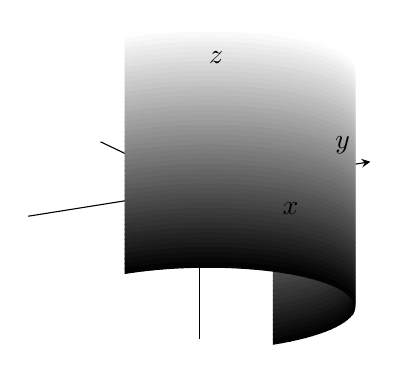
\begin{tikzpicture}
            \begin{axis}[
                view={60}{20},
                axis lines=middle,
                xlabel={$x$}, ylabel={$y$}, zlabel={$z$},
                xmin=-4, xmax=4, ymin=-2.5, ymax=2.5, zmin=-2.5, zmax=2.5,
                ticks=none
            ]
            \addplot3[
                samples=50,
                domain=0:pi,
                y domain=-2:2,
                surf,
                shader=flat,
                colormap/blackwhite
            ]
            (
                {3 * cos(deg(x))},
                {2 * sin(deg(x))},
                {y}
            );
            \end{axis}
            \end{tikzpicture}
    \end{center}

    \item[(b)] Given parameterization:
    \[ \vec{r}(u, v) = \langle u \sin v, u^2, u \cos v \rangle, \quad 0 \leq u \leq 3, \quad 0 \leq v \leq 2\pi \]

    \[ x(u, v) = u \sin v, \quad y(u, v) = u^2, \quad z(u, v) = u \cos v \]

    \[  \sin v = \frac{x}{u}, \quad \cos v = \frac{z}{u} \]

    \[ \left( \frac{x}{u} \right)^2 + \left( \frac{z}{u} \right)^2 = 1 \]

    \[ x^2 + z^2 = u^2 \]

    \[ x^2 + z^2 = y \]

    \begin{center}
        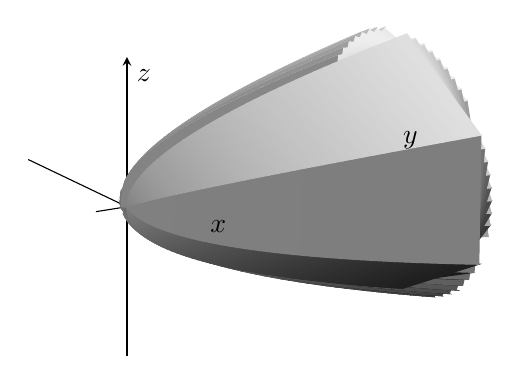
\begin{tikzpicture}
            \begin{axis}[
                view={60}{20},
                axis lines=middle,
                xlabel={$x$}, ylabel={$y$}, zlabel={$z$},
                xmin=-3.5, xmax=3.5, ymin=-1, ymax=10, zmin=-3.5, zmax=3.5,
                ticks=none
            ]
            \addplot3[
                samples=50,
                domain=0:3,
                y domain=0:360,
                surf,
                shader=flat,
                colormap/blackwhite
            ]
            (
                {x * sin(deg(y))},
                {x^2},
                {x * cos(deg(y))}
            );
            \end{axis}
            \end{tikzpicture}
    \end{center}

\end{enumerate}




\qs{}{
    Consider the surface \( S \) described by \( x - 4y^2 - z^2 + 3 = 0 \).
    \begin{enumerate}
        \item[(a)] Find a parametrization of \( S \) of the form \( \vec{r}_1(u, v) = \langle f(u, v), u, v \rangle \). Give the domain for your parametrization.
        \item[(b)] Find a parametrization of \( S \) of the form \( \vec{r}_2(u, v) = \langle v, f(v) \cos u, g(v) \sin u \rangle \). Give the domain for your parametrization.
        \item[(c)] How must we restrict the parameters \( (u, v) \) in part (a) if we only want the part of \( S \) that lies in front of the \( yz \)-plane, i.e., where \( x \geq 0 \)?
        \item[(d)] How must we restrict the parameters \( (u, v) \) in part (b) if we only want the part of \( S \) that lies in front of the \( yz \)-plane?
    \end{enumerate}
}


\begin{enumerate}
    \item[(a)]
    \[ x = 4y^2 + z^2 - 3. \]    
    \[ \vec{r}_1(u, v) = \langle 4u^2 + v^2 - 3, u, v \rangle. \]    
    \[ (u, v) \in \mathbb{R}^2. \]
    
    \item[(b)] 
    \[ \vec{r}_2(u, v) = \langle v, f(v) \cos u, g(v) \sin u \rangle \] 
    \[ x = v \quad  y = f(v) \cos u \quad  z = g(v) \sin u \] 
    \[ v - 4\left[f(v) \cos u\right]^2 - \left[g(v) \sin u\right]^2 + 3 = 0. \]
    \[ v - 4f(v)^2 \cos^2 u - g(v)^2 \sin^2 u + 3 = 0. \]
    \[ 4f(v)^2 = k \quad \text{and} \quad g(v)^2 = k \]
    \[ k = v + 3 \]
    \[ f(v) = \frac{1}{2} \sqrt{v + 3}, \quad g(v) = \sqrt{v + 3}. \]    
    \[ \vec{r}_2(u, v) = \left\langle v, \frac{1}{2} \sqrt{v + 3} \cos u, \sqrt{v + 3} \sin u \right\rangle \]    
    \[ v \geq -3, \quad u \in \mathbb{R} \]
    
    \item[(c)] 
    
    \[ x = 4u^2 + v^2 - 3 \geq 0 \]    
    \[ 4u^2 + v^2 \geq 3 \]
        
    \item[(d)] 
    \[ v \geq 0. \]
        
    \[ v \geq 0, \quad u \in \mathbb{R} \]
\end{enumerate}


\qs{}{
    Find parametric equations for each of the following surfaces.
    \begin{enumerate}
        \item[(a)] The part of the plane \( z = x + 3 \) that lies inside the cylinder \( x^2 + y^2 = 1 \).
        \item[(b)] The surface obtained by rotating the curve \( x = 4y^2 - y^4 \), \( -2 \leq y \leq 2 \) about the \( y \)-axis.
        \item[(c)] The ellipsoid \( \frac{x^2}{4} + 4y^2 + \frac{z^2}{9} = 1 \).
    \end{enumerate}
}

\subsection*{Part (a)}

    \[ x = r \cos\theta, \quad y = r \sin\theta, \]
    \[ r \in [0, 1] \quad  \text{and} \theta \in [0, 2\pi) \]

    \[ z = r \cos\theta + 3. \]

    \[ \begin{cases}
    x = r \cos\theta, \\
    y = r \sin\theta, \\
    z = r \cos\theta + 3,
    \end{cases} \]
    \[ 0 \leq r \leq 1 \quad  \text{and} \quad  0 \leq \theta < 2\pi \].

\subsection*{Part (b)}
    \[ \begin{cases}
    x = [4y^2 - y^4] \cos\theta, \\
    z = [4y^2 - y^4] \sin\theta, \\
    y = y, \end{cases} \]
    \[ -2 \leq y \leq 2 \quad \text{and}  0 \leq \theta < 2\pi \] 
    \[ \begin{cases}
    x = \left(4y^2 - y^4\right) \cos\theta, \\
    y = y, \\
    z = \left(4y^2 - y^4\right) \sin\theta,
    \end{cases} \]
    \[ -2 \leq y \leq 2 \quad \text{and} 0 \leq \theta < 2\pi \].


\subsection*{Part (c)}

\textbf{Solution:}

    \[ X = \dfrac{x}{2}, \quad Y = 2y, \quad Z = \dfrac{z}{3} \]
    \[ X^2 + Y^2 + Z^2 = 1 \]

    \[ \begin{cases}
    X = \sin\phi \cos\theta, \\
    Y = \sin\phi \sin\theta, \\
    Z = \cos\phi,
    \end{cases} \]
    \[ \phi \in [0, \pi] \quad \text{and} \quad  \theta \in [0, 2\pi) \]

    \[ \begin{cases}
    x = 2X = 2\sin\phi \cos\theta, \\
    y = \dfrac{Y}{2} = \dfrac{1}{2}\sin\phi \sin\theta, \\
    z = 3Z = 3\cos\phi.
    \end{cases} \]

    \[
    \begin{cases}
    x = 2 \sin\phi \cos\theta, \\
    y = \dfrac{1}{2} \sin\phi \sin\theta, \\
    z = 3 \cos\phi,
    \end{cases} \]
    \[ 0 \leq \phi \leq \pi \quad \text{and} \quad 0 \leq \theta < 2\pi \] 



\qs{}{
    Find the tangent plane to the parametric surface \( \vec{r}(u, v) = \langle u \sin v, u^2, u \cos v \rangle \) at the point where \( u = 1 \) and \( v = \frac{\pi}{3} \). Write the plane both in the vector form \( \vec{r}(u, v) = \vec{r}_0 + u \vec{a} + v \vec{b} \) and in the form \( ax + by + cz = d \).
}

\sol{
    \[ \vec{r}_0 = \vec{r}(1, \tfrac{\pi}{3}) = \left\langle 1 \cdot \sin \tfrac{\pi}{3},\ 1^2,\ 1 \cdot \cos \tfrac{\pi}{3} \right\rangle = \left\langle \tfrac{\sqrt{3}}{2},\ 1,\ \tfrac{1}{2} \right\rangle. \]
    \[ \vec{r}_u(u, v) = \left\langle \sin v,\ 2u,\ \cos v \right\rangle \]
    \[ \vec{r}_v(u, v) = \left\langle u \cos v,\ 0,\ -u \sin v \right\rangle \]
    \[ \vec{r}_u(1, \tfrac{\pi}{3}) = \left\langle \sin \tfrac{\pi}{3},\ 2,\ \cos \tfrac{\pi}{3} \right\rangle = \left\langle \tfrac{\sqrt{3}}{2},\ 2,\ \tfrac{1}{2} \right\rangle, \]
    \[ \vec{r}_v(1, \tfrac{\pi}{3}) = \left\langle 1 \cdot \cos \tfrac{\pi}{3},\ 0,\ -1 \cdot \sin \tfrac{\pi}{3} \right\rangle = \left\langle \tfrac{1}{2},\ 0,\ -\tfrac{\sqrt{3}}{2} \right\rangle. \]
    \[ \vec{r}(s, t) = \vec{r}_0 + s\,\vec{r}_u(1, \tfrac{\pi}{3}) + t\,\vec{r}_v(1, \tfrac{\pi}{3}) \]
    \[ \vec{r}(s, t) = \left\langle \tfrac{\sqrt{3}}{2},\ 1,\ \tfrac{1}{2} \right\rangle + s \left\langle \tfrac{\sqrt{3}}{2},\ 2,\ \tfrac{1}{2} \right\rangle + t \left\langle \tfrac{1}{2},\ 0,\ -\tfrac{\sqrt{3}}{2} \right\rangle. \]
    \[ \vec{n} = \vec{r}_u(1, \tfrac{\pi}{3}) \times \vec{r}_v(1, \tfrac{\pi}{3}) = \begin{vmatrix}
    \mathbf{i} & \mathbf{j} & \mathbf{k} \\
    \tfrac{\sqrt{3}}{2} & 2 & \tfrac{1}{2} \\
    \tfrac{1}{2} & 0 & -\tfrac{\sqrt{3}}{2}
    \end{vmatrix}. \]
    \[ \vec{n} = \left( -\sqrt{3},\ 1,\ -1 \right) \]

    \[ \vec{n} \cdot (\vec{r} - \vec{r}_0) = 0. \]
    \[ -\sqrt{3}(x - \tfrac{\sqrt{3}}{2}) + 1(y - 1) - 1(z - \tfrac{1}{2}) = 0 \]
    \[ -\sqrt{3}x + y - z + \left( \tfrac{3}{2} - 1 + \tfrac{1}{2} \right) = 0, \]
    \[ -\sqrt{3}x + y - z + 1 = 0. \]
    \[ \sqrt{3}x - y + z = 1 \]
    \[ \sqrt{3}\,x\ -\ y\ +\ z\ =\ 1 \]
    \[ \vec{r}(s, t) = \left\langle \tfrac{\sqrt{3}}{2},\ 1,\ \tfrac{1}{2} \right\rangle + s \left\langle \tfrac{\sqrt{3}}{2},\ 2,\ \tfrac{1}{2} \right\rangle + t \left\langle \tfrac{1}{2},\ 0,\ -\tfrac{\sqrt{3}}{2} \right\rangle. \]
    \[ \sqrt{3}\,x\ -\ y\ +\ z\ =\ 1 \]}

\end{document}